\documentclass[aspectratio=169,10pt]{beamer}
% Course-local adaptation of the copied Sorbonne Beamer reference assets.
% The files in template/assets/ are preserved verbatim from the reference copy.
\usepackage[T1]{fontenc}
\usepackage[utf8]{inputenc}
\usepackage{lmodern}
\usepackage{amsmath,amssymb,mathtools}
\usepackage{booktabs}
\usepackage{graphicx}
\usepackage{tikz}
\usetikzlibrary{arrows.meta,positioning,calc}
\usepackage{ragged2e}
\usepackage{hyperref}
\definecolor{bleu}{RGB}{0,129,188}
\definecolor{rouge}{RGB}{238,50,78}
\definecolor{orange}{RGB}{255,100,0}
\definecolor{vert}{RGB}{0,157,87}
\definecolor{dp}{RGB}{181,73,60}
\usetheme{Frankfurt}
\useoutertheme[subsection=false,shadow]{miniframes}
\usepackage{template/assets/beamercolorthemeEwen}
\usepackage{template/assets/beamerouterthemeEwen}
\usepackage{template/assets/beamerhighlight}
\usefonttheme{serif}
\setbeamerfont{title like}{shape=\scshape}
\setbeamerfont{frametitle}{shape=\scshape}
\setbeamercolor{frametitle}{fg=dp,bg=white}
\setbeamercolor{structure}{fg=black}
\setbeamercolor{alerted text}{fg=dp}
\setbeamertemplate{navigation symbols}{}
\setbeamertemplate{items}[triangle]
\setbeamertemplate{footline}{%
  \leavevmode\hbox{\begin{beamercolorbox}[wd=1\paperwidth,ht=2.25ex,dp=1ex,center]{title in head/foot}
  \hfill\hspace*{8em}\insertshorttitle\hspace*{2em}\insertframenumber{} / \inserttotalframenumber\hspace*{1ex}
  \end{beamercolorbox}}\vskip0pt}
\newcommand{\key}[1]{\textcolor{dp}{\textbf{#1}}}
\AtBeginSection[]{\begin{frame}{Plan}\tableofcontents[currentsection,hideallsubsections]\end{frame}}

\title[BTM -- Session 2]{A Production Economy}
\subtitle{RBC structure, rational expectations and Dynare}
\author[Gauthier Vermandel]{Gauthier Vermandel}
\institute{Paris-Dauphine -- PSL}
\date{12 November 2026}
\begin{document}
\begin{frame}\titlepage\end{frame}
\begin{frame}{Session objective}\begin{itemize}\item Build the core equilibrium conditions of a stochastic production economy.\item See how rational-expectations models are solved and diagnosed.\item Translate an economic model into readable Dynare code.\end{itemize}\vfill\key{Handout:} Chapter 2 \quad \key{Code:} \texttt{chap2/codes/}\end{frame}
\section{Production economy}
\begin{frame}{The RBC benchmark}
\centering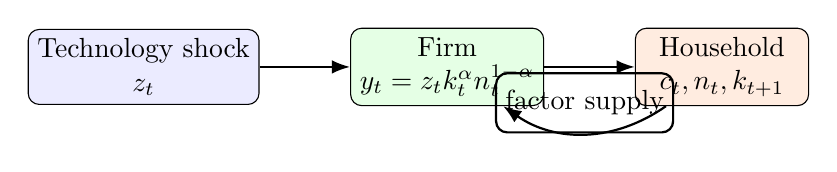
\begin{tikzpicture}[node distance=1.15cm,>=Latex,every node/.style={draw,rounded corners,align=center,minimum width=2.2cm,minimum height=.75cm}]
\node[fill=blue!8] (shock) {Technology shock\\$z_t$};\node[fill=green!10,right=of shock] (firm) {Firm\\$y_t=z_t k_t^\alpha n_t^{1-\alpha}$};\node[fill=orange!12,right=of firm] (hh) {Household\\$c_t,n_t,k_{t+1}$};
\draw[->,thick] (shock)--(firm);\draw[->,thick] (firm)--(hh);\draw[->,thick,bend left=35] (hh) to node[above]{factor supply} (firm);\end{tikzpicture}
\vfill Resource constraint: \(c_t+i_t=y_t\), with \(k_{t+1}=(1-\delta)k_t+i_t\).\end{frame}
\begin{frame}{Equilibrium conditions organize the model}
\begin{columns}[T]\begin{column}{.48\textwidth}\textbf{Household}
\[u_c(c_t,n_t)=\beta\mathbb E_t\{u_c(c_{t+1},n_{t+1})(r_{t+1}+1-\delta)\}\]
\[-u_n(c_t,n_t)=u_c(c_t,n_t)w_t\]
\end{column}\begin{column}{.48\textwidth}\textbf{Firm}
\[r_t=\alpha z_t k_t^{\alpha-1}n_t^{1-\alpha}\]
\[w_t=(1-\alpha)z_t k_t^\alpha n_t^{-\alpha}\]
\end{column}\end{columns}\vfill\key{Discipline:} every variable needs an equation, a timing convention and a unit.\end{frame}
\section{Solution}
\begin{frame}{Linear rational expectations form}
After approximation, many models take the form \[A\,\mathbb E_t x_{t+1}=B x_t+C x_{t-1}+D\varepsilon_t.\]
\begin{itemize}\item Predetermined states carry history.\item Forward-looking controls respond to expected future states.\item A unique stable solution requires the appropriate number of unstable roots.\end{itemize}\end{frame}
\begin{frame}{What an impulse response can -- and cannot -- tell us}
\begin{columns}\begin{column}{.55\textwidth}\begin{itemize}\item An IRF is a conditional model experiment, not a causal estimate by itself.\item Its shape reflects parameter values, shock normalization and solution method.\item Compare mechanisms, not only peak responses.\end{itemize}\end{column}\begin{column}{.38\textwidth}\begin{block}{Checklist}Sign? Units? Horizon? Shock size? Stability? Plausible transmission?\end{block}\end{column}\end{columns}\end{frame}
\section{Dynare}
\begin{frame}[fragile]{A readable Dynare skeleton}\small\begin{verbatim}
var c k y n z;
varexo e;
parameters beta alpha delta rho sigma_e;

model;
  y = exp(z)*k(-1)^alpha*n^(1-alpha);
  c + k = y + (1-delta)*k(-1);
  1/c = beta*(1/c(+1))*(alpha*y(+1)/k);
  z = rho*z(-1) + e;
end;
\end{verbatim}
\vfill\key{Rule:} code mirrors the economic model; comments document transformations and timing.
\end{frame}
\begin{frame}{Dynare workflow}\centering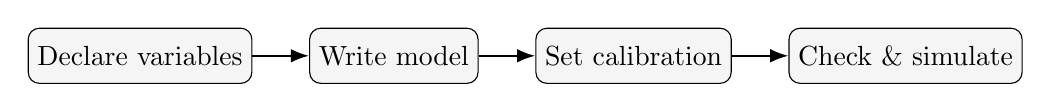
\begin{tikzpicture}[node distance=.72cm,>=Latex,every node/.style={draw,rounded corners,align=center,minimum width=2.0cm,minimum height=.7cm,fill=gray!8}]
\node (a) {Declare variables};\node[right=of a] (b) {Write model};\node[right=of b] (c) {Set calibration};\node[right=of c] (d) {Check \& simulate};\draw[->,thick] (a)--(b);\draw[->,thick] (b)--(c);\draw[->,thick] (c)--(d);\end{tikzpicture}
\vfill\begin{itemize}\item Read Dynare messages; do not treat warnings as decorative.\item Generated folders and output are reproducible and intentionally ignored by Git.\end{itemize}\end{frame}
\section{Takeaways}
\begin{frame}{Takeaways and preparation}\begin{itemize}\item The RBC model connects preferences, technology and resource feasibility.\item Rational expectations impose solution and determinacy requirements.\item Dynare is valuable when the code remains a transparent representation of the model.\end{itemize}\vfill\key{Before Session 3:} run \texttt{basicRBC.mod}; retain the code, not generated outputs.\end{frame}
\end{document}
